\chapter{Ponderado de normales}
\label{chap:ponderadoNormales}
Se desea encontrar una forma de asignar las normales a la superficie que se usarán para hacer la iluminación. La manera propuesta sera crear primero una superficie implícita que envuelva la aproximación poligonal $\mathcal{A}_{\tau}$. La superficie implícita esta formada por funciones base, por lo tanto cada una de estas contribuye a la superficie y contribuye también a la forma como se van a modificar las normales. En este sentido en este trabajo entenderemos como \emph{ponderación} al proceso de ir sumando vectores que modifican la dirección de un vector normal. Dado que para hacer cálculos de iluminación los vectores deben ser unitarios, después de la ponderación hacemos un postproceso que nos asegure solo usar vectores unitarios. Por esta razón se hace énfasis en que las funciones base cambian \emph{la dirección} del vector normal.

\section{Representación implícita de superficies}
\label{sec:repImplicita}
Tradicionalmente en las GC hay dos formas de modelar superficies en el espacio $\mathbb{R}^3$ \cite{Blinn:metaballs}. Una de ellas es tener la superficie definida de manera paramétrica $s(\mu,\nu)$. Por lo tanto es posible crear una aproximación por medio de polígonos calculando los vértices mediante incrementos constantes en los parámetros.

Otra forma, es la llamada representación implícita. Que consiste en encontrar las soluciones de la siguiente ecuación:
\begin{equation}
 f(\textbf{x}) = 0,
\label{ec:supImplicita}
\end{equation}
donde $\textbf{x} \in \mathbb{R}^3$. Aunque ya se habían estudiado las superficies producidas por funciones de segundo grado, Blinn propuso una manera de generalizar estas superficies en \cite{Blinn:metaballs}. La idea de Blinn tenía el objetivo de representar estructuras moleculares donde los átomos se combinan con otros con transiciones graduales. Esta representación ha sido adoptada para realizar modelado de objetos orgánicos y funciones topológicamente muy complicadas. En el trabajo original una molécula es representada aproximadamente por medio de la combinación lineal de funciones suaves. En dicha representación, cada $j$-esimo átomo de la molécula es representado por una función suave $b_j$ ponderada por un coeficiente $c_j$ y centrada en el punto $\textbf{p}_j$ de la siguiente forma
\begin{equation}
 g(\textbf{x}) \approx \sum \limits_{j = 1}^{j} c_j b_j(\textbf{x} - \textbf{p}_j).
\label{ec:modeloBlobby}
\end{equation}

Blinn propuso utilizar la siguiente función $b$ (radialmente simétrica):
\begin{equation}
 b(\alpha ; r) = e^{-\alpha r},
\label{ec:blobBlinn}
\end{equation}
donde $r$ es la distancia de $\textbf{x}$ al punto $\textbf{p}_i$ donde está centrada la función y $\alpha$ representa un parámetro de forma de la función (el ancho) .

Para llevar a cabo la visualización de \eqref{ec:modeloBlobby}, se define un umbral o isovalor $t$,que se aproxima por poligonalización o por \emph{raycasting}.

\subsection{Las funciones Kaiser-Bessel generalizadas (\textit{blobs})}

La aproximación \eqref{ec:modeloBlobby} también sirve para modelar funciones de densidad en el área de reconstrucción a partir de proyecciones (un problema inverso cuyo ejemplo mas típico son los instrumentos médicos que realizan tomografías \cite{tomografyBook}). En particular son usados en aquellos métodos basados en expansiones en series de funciones base. En este campo también se han usado varias funciones base tales como vóxeles. Pero una función base que ha resultado en buenas aproximaciones son las funciones Kaiser-Bessel generalizadas \cite{BlobsMate}, definidas como:
\begin{equation}
\label{ec:blob}
 b(m, \alpha, a; r) = \begin{cases}
            \dfrac{ I_m \left(  \alpha \sqrt{1 - \left( \frac{r}{a} \right) ^2 }  \right) } {I_m(\alpha)} \left( \sqrt{1 - \left( \frac{r}{a} \right) ^2 }  \right)^m, & \text{si $0 \leq r \leq a$,} \\
                    0, & \text{en otro caso,} \\
            \end{cases}
\end{equation}
en donde $r$ es la distancia radial al centro del blob, $I_m$ es la función Bessel modificada de orden $m$, $a$ determina el soporte y $\alpha$ es el parámetro que controla la forma de la función. 

La elección de las funciones Kaiser-Bessel generalizadas se debe a sus propiedades adecuadas para el área de procesamiento de imágenes, tales como la continuidad en el soporte finito y su rápida tasa de desvanecimiento en su espectro (algo que se considera como ancho de banda limitado en la practica), ver Figura \ref{fig:blobSpectre}. De hecho, estas funciones son muy conocidas en al área de procesamiento de señales donde son utilizadas típicamente como ventanas (\emph{windows} en ingles). De ahora en adelante al usar el termino \emph{blob} nos referiremos a la función base de \eqref{ec:blob}.

\begin{figure}[htp]
 \centering
  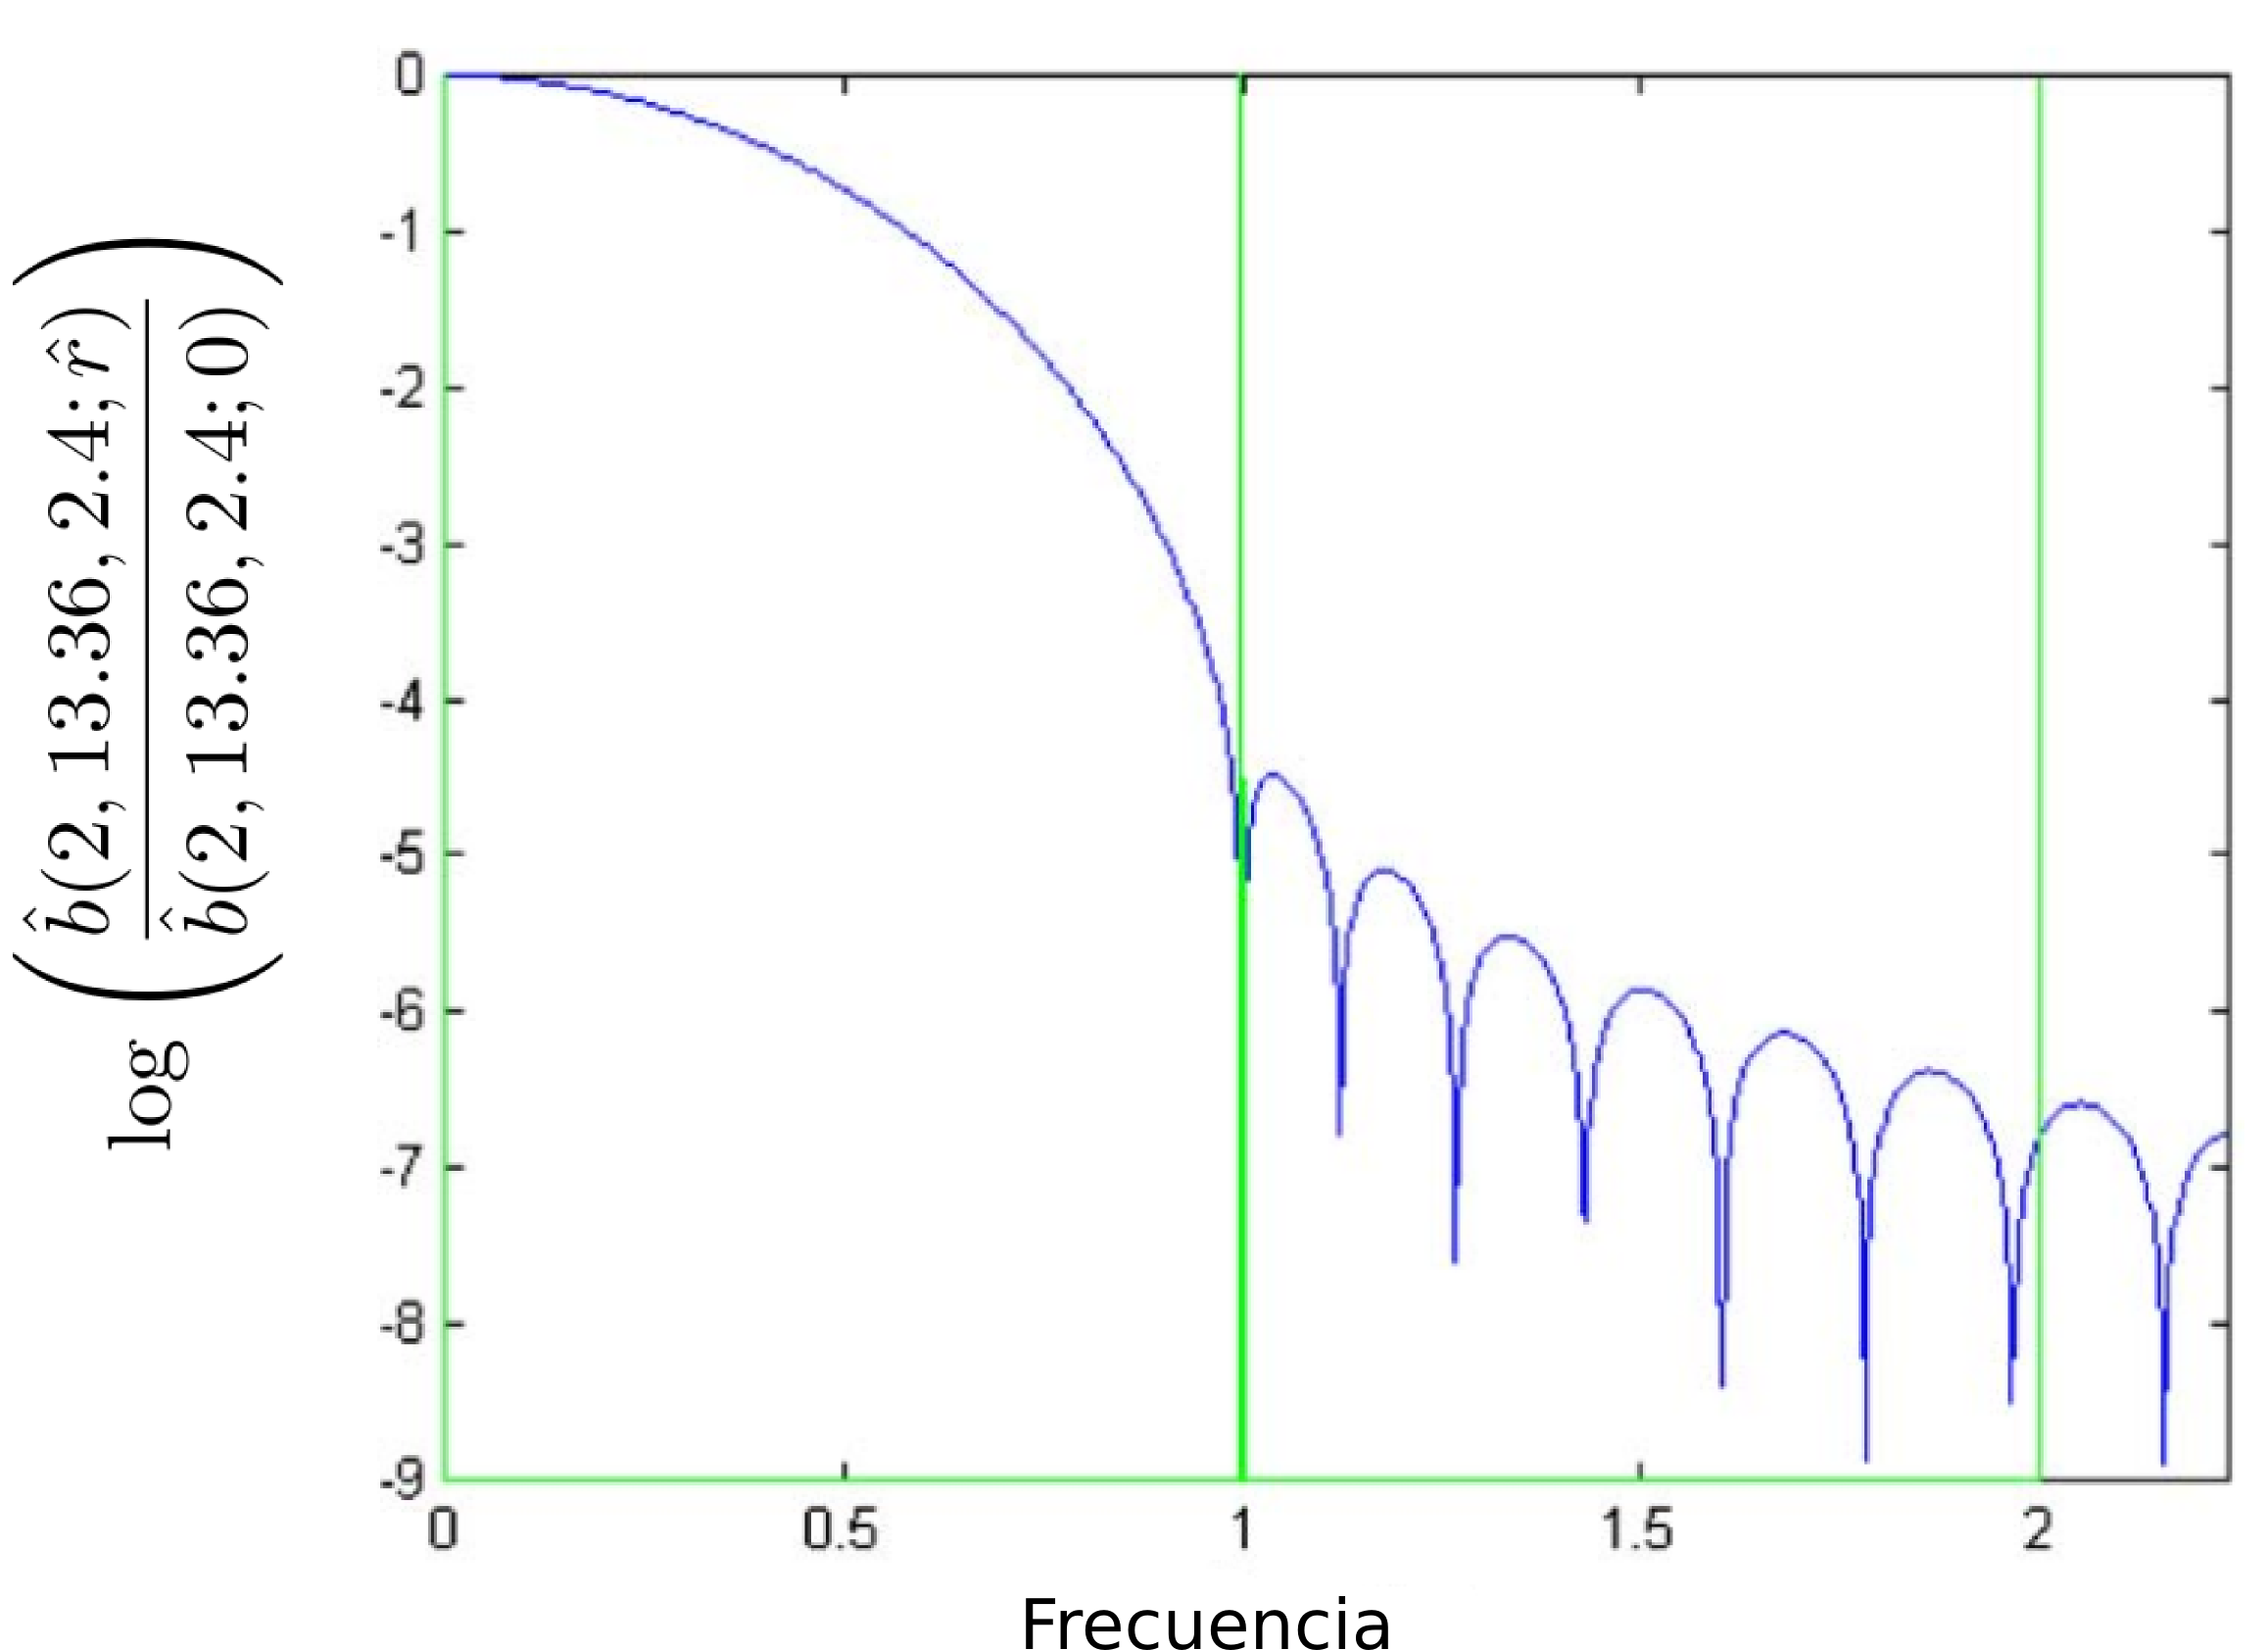
\includegraphics[scale=0.9]{img/cap02/blobSpectre}
  \caption[Espectro del blob en escala logarítmica]{Aquí se gráfica la magnitud de la transformada de Fourier del blob (espectro) en escala logarítmica contra la distancia radial $\hat{r}$ al centro del blob (frecuencia).}
  \label{fig:blobSpectre}
\end{figure}
